\documentclass[a3paper]{standalone}
\usepackage{tikz}
\usetikzlibrary{shapes, arrows, positioning}
\usepackage{amsmath}

\begin{document}
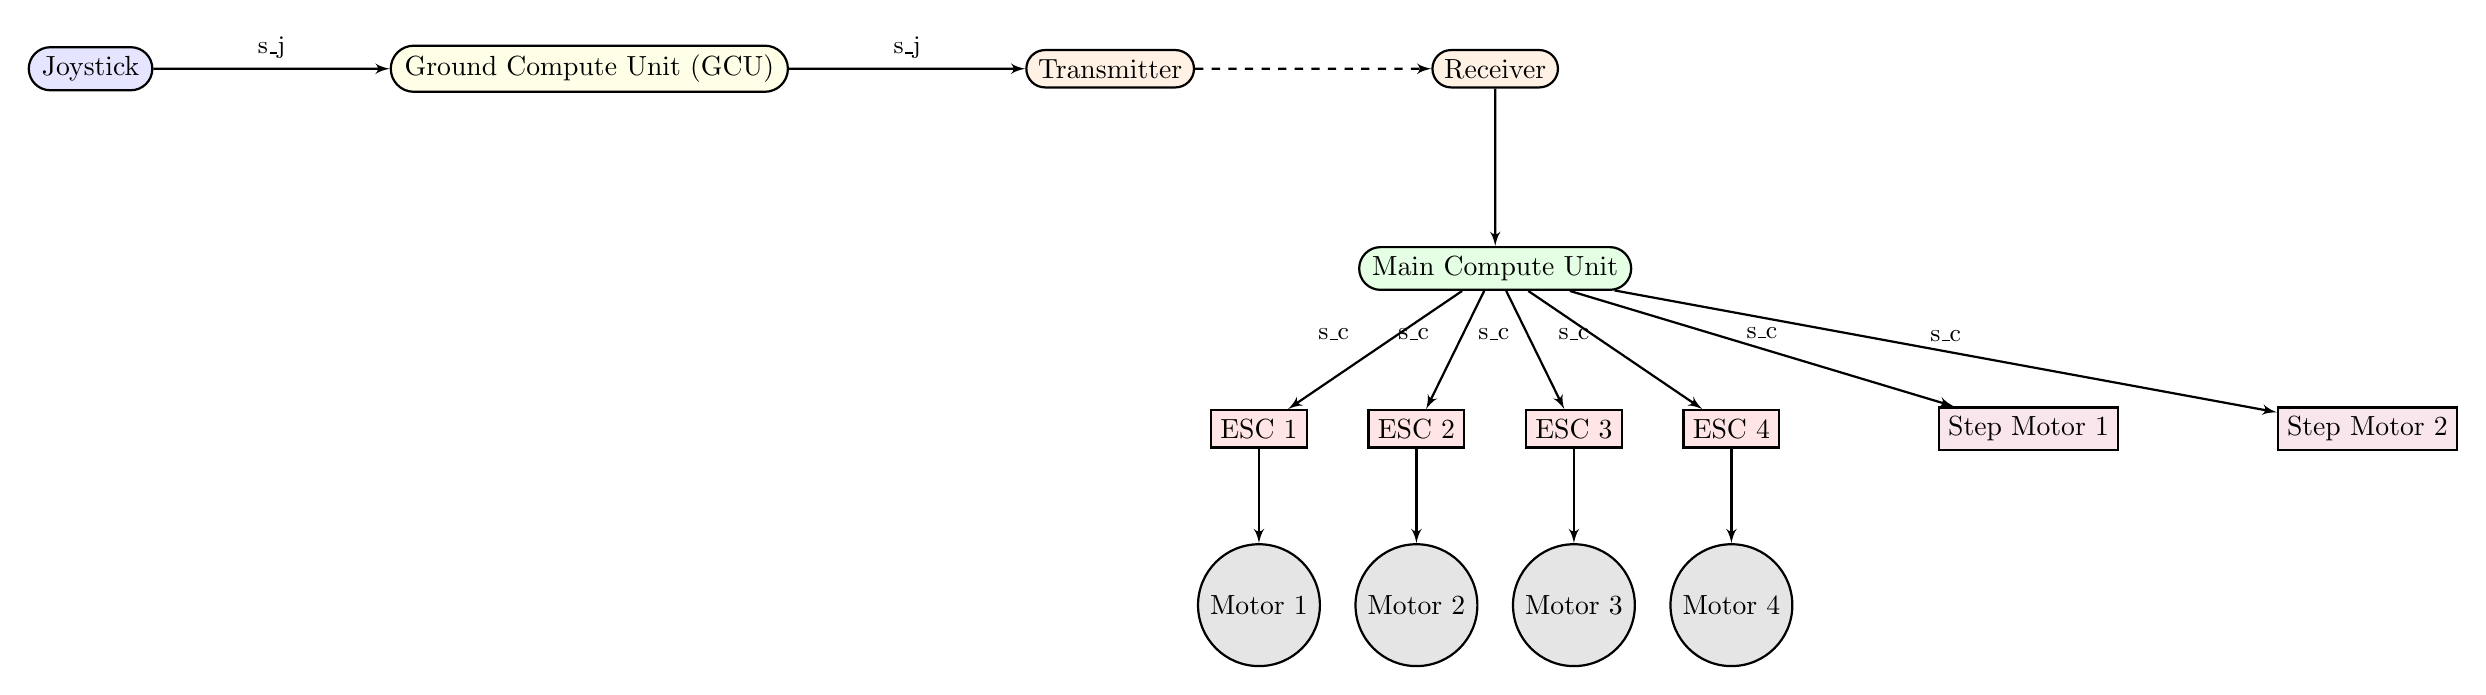
\begin{tikzpicture}[node distance=2cm, auto, >=latex', thick]
  % Nodes
  \node[draw, rounded rectangle, fill=blue!10] (joystick) {Joystick};
  \node[draw, rounded rectangle, right=3cm of joystick, fill=yellow!10] (gcu) {Ground Compute Unit (GCU)};
  \node[draw, rounded rectangle, right=3cm of gcu, fill=orange!10] (tx) {Transmitter};
  \node[draw, rounded rectangle, right=3cm of tx, fill=orange!10] (rx) {Receiver};
  \node[draw, rounded rectangle, below=2cm of rx, fill=green!10, minimum width=3cm] (mcu) {Main Compute Unit};

  % ESCs and Motors
  \foreach \i in {1,...,4} {
    \node[draw, rectangle, below=1.5cm of mcu, xshift={(\i-2.5)*2cm}, fill=red!10] (esc\i) {ESC \i};
    \node[draw, circle, below=1.2cm of esc\i, fill=gray!20] (motor\i) {Motor \i};
    \draw[->] (mcu) -- node[left, font=\small, xshift=-2mm, yshift=2mm]{s\_c} (esc\i);
    \draw[->] (esc\i) -- (motor\i);
  }

  % Step Motors
  \node[draw, rectangle, right=2cm of esc4, fill=purple!10] (step1) {Step Motor 1};
  \node[draw, rectangle, right=2cm of step1, fill=purple!10] (step2) {Step Motor 2};
  \draw[->] (mcu) -- node[above, font=\small]{s\_c} (step1);
  \draw[->] (mcu) -- node[above, font=\small]{s\_c} (step2);

  % Connections
  \draw[->] (joystick) -- node[above, font=\small]{s\_j} (gcu);
  \draw[->] (gcu) -- node[above, font=\small]{s\_j} (tx);
  \draw[->, dashed] (tx) -- (rx);
  \draw[->] (rx) -- (mcu);
\end{tikzpicture}

% Legende
\vspace{1cm}
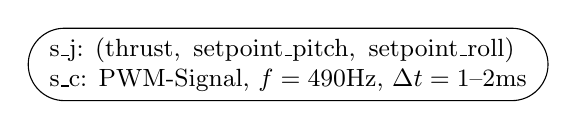
\begin{tikzpicture}
  \node[draw, fill=white!90, rounded rectangle, font=\small, align=left] at (0,0) {
    s\_j: $(\text{thrust},\ \text{setpoint\_pitch},\ \text{setpoint\_roll})$\\
    s\_c: PWM-Signal, $f=490$Hz, $\Delta t=1$--$2$ms
  };
\end{tikzpicture}
\end{document}